\begin{figure*}[t]
    \centering
    \begin{subfigure}[b]{0.48\textwidth}
        \centering
        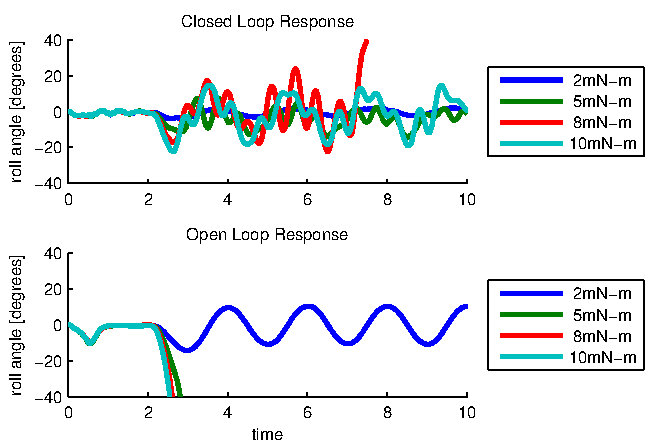
\includegraphics[width = \textwidth]{figures/torques_small.pdf}
        \caption{1 Hz}
        \label{fig:results1Hz}
    \end{subfigure}
    \quad
    \begin{subfigure}[b]{0.48\textwidth}
        \centering
        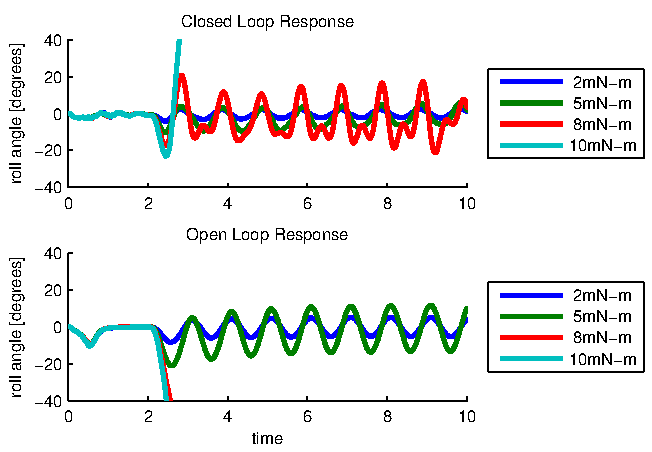
\includegraphics[width = \textwidth]{figures/torques_small2.pdf}
        \caption{2 Hz}
        \label{fig:results2Hz}
    \end{subfigure}
    \caption{Closed and open loop sytem response to sinusoidal disturbance torques at two frequencies and various amplitiudes. Disturbance starts at the two second mark.}
\end{figure*}

We implemented the controller described in the previous section in order to regulate the height and roll of the water runner robot in simulation. To tune the gains on our virtual model, we used the Ziegler-Nichols Method as our virtual model is simply a PID controller in task-space. We assigned $\omega_0$ by averaging the leg frequencies used in the last time step.

Figure~\ref{fig:results1Hz} shows the closed and open-loop roll motion responses of the system subject to 1 Hz sinusoidal torques of various amplitude acting on the robot's center of mass in the roll direction. We do not show the height resposne, as the robot generally sinks only after reaching an extreme roll angle. It is evident from this figure that the controller is able to significantly reduce the effects of these disturbances on the robot as it is able to stabilize the robot against 2, 5, and 10 mN-m disturbances whereas the open loop system is unstable for all but the smallest amplitude disturbance. When we compare the responses of the system to the 2mN-m torque we see that the amplitude of osccilations is reduced in closed loop system.

Figure~\ref{fig:results2Hz} shows the closed and open-loop responses of the system to sinusoidal disturbances with the same amplitudes as before, but at a a higher frequency of 2Hz. The open loop system fares better in this test, perhaps because the higher frequncy waves impose smaller impulses on the system than the lower frequncy waves do. However, the performance of the closed loop system is still superior as, unlike the open loop system, it is stable against 8mN-m waves and it exhibits smaller oscillations than the open-loop system at disturbance frequencies for which both systems are stable.

\begin{comment}
Finally, figure~\ref{fig:omega0} shows the variation in leg frequencies that can be achieved within the nullspace of the dynamical system. These figures show the time-varying velocities of the robot's four legs as the controller attempts to stabilize the sytem against an 8mN-m, 2Hz disturbance torque. Figure~\ref{fig:omega25} shows the leg velocities produced using a 25/75 mix between the averaging scheme that promotes differences in upwards and downwards leg speeds and the averaging scheme that promotes constant leg speeds within a cycle. In contrast, figure~\ref{fig:omega75} shows the leg velocitites acheived using a 75/25 mix of these two averaging schemes. It is evident that the legs velocities in the second plot switch between upwards and downwards velocities that are more disparate than those in the first figure. However, both of these leg velocity profiles produce similar robot motions and successfully reject the input disturbance.

\begin{figure*}[t]
    \centering
    \begin{subfigure}[b]{0.48\textwidth}
        \centering
        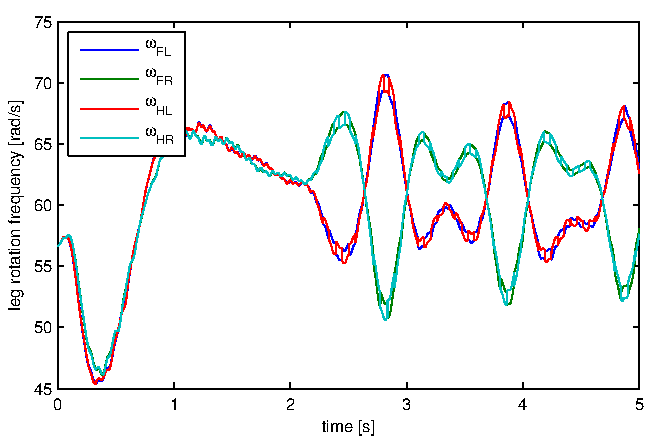
\includegraphics[width = \textwidth]{figures/omega25.pdf}
        \caption{$\omega_0$ set according to 25/75 mix of averaging schemes.}
        \label{fig:omega25}
    \end{subfigure}
    \quad
    \begin{subfigure}[b]{0.48\textwidth}
        \centering
        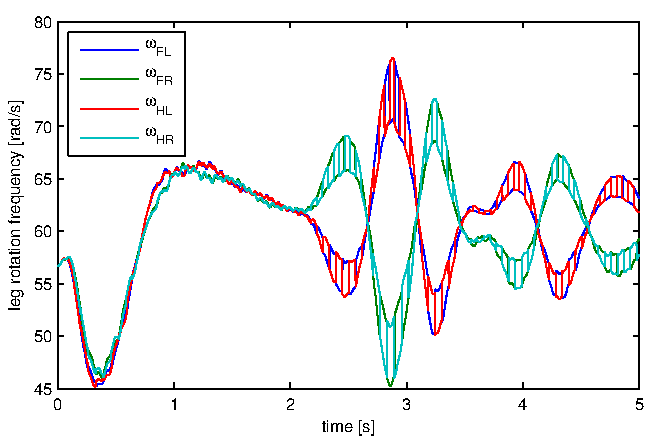
\includegraphics[width = \textwidth]{figures/omega75.pdf}
        \caption{$\omega_0$ set according to 75/25 mix of averaging schemes.}
        \label{fig:omega75}
    \end{subfigure}
    \caption{Leg velocities found via two different averaging schemes that either promote differences in upwards and downwards leg speeds or promote constant leg speeds on each side of the robot.}
    \label{fig:omega0}
\end{figure*}
\end{comment}
